\section{Lecture 4: Stabilizer QEC and CSS Codes - 11 February 2026}
Outline:
\begin{enumerate}[label=(\Roman*)]
    \item Stabilizers continued
    \item Stabilizer code criteria 
    \item Classical linear codes 
    \item CSS Codes
\end{enumerate}
Last time: code $\{\ket{\psi_l}\}$, errors $\{E_k\}$ \\
\begin{equation}
    \braket{\psi_l | E_a^\dagger E_b |\psi_m} = \alpha_{ab} \delta_{lm}
\end{equation}

\subsection{Stabilizers}
Recall: Stablizers:
\begin{equation}
    S = \{g \in G_n \,|\, g\ket{\psi} = \ket{\psi}, \forall \ket{\psi} \in V_s \}
\end{equation}
and by convention, $-I \notin S$. 
\begin{example}
    Stablizer Examples:
    \begin{itemize}
        \item $V_s = \{\ket{000}, \ket{111}\} \Rightarrow S = \langle ZZI, IZZ \rangle$
        \item $S = \{X,Y\} \Rightarrow V_s = \emptyset$ since $S$ is an ill-formed stabilizer set because $X$ and $Y$ do not commute with each other and all stabilizers must commute with each other 
        \item $V_s = \{(\ket{000} + \ket{111})^{\otimes 3}, (\ket{000} + \ket{111})^{\otimes 3}\} \Rightarrow S = \langle Z_1Z_2, Z_2Z_3, Z_4Z_5,\ldots, X_1X_2X_3X_4X_5X_6, \ldots \rangle$ \\
        In this case $n = 9, k= 1$. The minimum amount of generators is $n-k = 8$ 
        \item $S = \langle XX\rangle \Rightarrow V_S = \{\ket{00} + \ket{11}, \ket{01} + \ket{10}\}$ \\ 
        In this case we have 1 stabilizer, 2 qubits, therefore, there must be 2 states.
        \item $V_s = \{\ket{0}\} \Rightarrow S = \langle Z\rangle$
        \item $V_s \{\ket{1}\} \Rightarrow S = \langle -Z \rangle$
        \item $V_s = \left\{\frac{\ket{01} + \ket{01}}{\sqrt{2}}, \ket{11}\right\} \Rightarrow S = \emptyset$
        \item $V_s = \left\{\frac{\ket{000} + \ket{111}}{\sqrt{2}}\right\} \Rightarrow S= \langle ZZI, IZZ, XXX\rangle$ since there's 1 state, 3 generators. 
    \end{itemize}
\end{example}


\subsection{Stabilizer Code Criteria}
\begin{definition}
    An $[[n,k]]$ stabilizer code $C(S)$ is th vector space stabilized by $S \subset G_n$, where 
    \begin{equation}
        S = \langle g_1, g_2, \ldots, g_{n-k} \rangle
    \end{equation}
\end{definition}
\begin{example}
    Shor Code: 
    $[[9,1]]$, $C(S) = \{(\ket{000} + \ket{111})^{\otimes 3}, (\ket{000} + \ket{111})^{\otimes 3}\}$
\end{example}
Observation: only 3 possible ways errors act on states inside the stabilizer space:
\begin{enumerate}
    \item $E \ket{\psi} \notin V_s$
    \item $E\ket{\psi} =\ket{\psi}$
    \item $E \ket{\psi} \neq \ket{\psi}$ but be in $V_s$
\end{enumerate}
\begin{theorem}
    Given errors $\{E_a\} \in G$ if $\exists g \in S$ s.t. $Eg= -gE$. We can find this to be true $\forall E = E_a^\dagger E_b$, then $\{E_a\}$ is correctable by the code $C(S)$
\end{theorem}
\textit{All we need to do is to get the code to correct something is find a generator which anticommutes with every single error. For every error that you have in the set (products thereof), we need to find some generator that anticommutes with it. If that's true then we can correct these errors. This is much simpler than Knil-Laflamme conditions.} 
\begin{proof}
    We want to show that the theorem above satisfies Knill-Laflamme. Sketch: 
    \begin{itemize}
        \item When $E = g \in S$, then $\braket{\psi_l|E|\psi_l} = \delta_{ij}$
        \item $\ket{\psi} \in C(S)$, $g \in S$, s.t. $Eg = -gE$, then $\braket{\psi|E|\psi} = \braket{\psi|Eg|\psi} = - \braket{\psi|gE|\psi} = -\braket{\psi|E|\psi} = 0$ (orthogonality criterion) 
        \item If $E_a = E_b$ then $E=E_aE_b = E_aE_a = I$ (non-deformation criterion)
    \end{itemize}
    Therefore, the theorem satisfies the Knill-Laflamme theorem. 
\end{proof}
\begin{definition}
    For $S = \langle g_1,g_2,\ldots,g_{n-k}\rangle$ and error $E$, $\forall l, l= 1, \ldots, n-k$, the error syndrome is 
    \begin{equation}
        \begin{cases}
            0 & \text{if } [g_l,E] = 0 \\
            1 & \text{otherwise}
        \end{cases}
    \end{equation}
\end{definition}
\begin{example} 
    Suppose $S = \langle IZZ, ZZI\rangle$
    \begin{itemize}
        \item if the error is $E = IXI$, the syndrome is $\{1,1\}$
        \item if the error is $E = XII$, the syndrome is $\{0,1\}$
    \end{itemize}
\end{example}
\begin{example}
    Suppose $S = \langle XX \rangle$, then as before $C(S) = \{\ket{00} + \ket{11}, \ket{01} + \ket{10}\}$. 
    \begin{itemize}
        \item Let $E=ZI$, syndrome $= \{1\}$
        \item Let $E=IZ$, syndrome $= \{1\}$
        \item Let $E=ZZ$, syndrome $= \{0\}$ since $ZZ$ and $XX$ commute 
        \begin{align}
            [XX,ZZ] &= (XZ\otimes XZ)(ZX \otimes ZX) - (ZX \otimes ZX)(XZ\otimes XZ)] \\
            &= (-iY\otimes -iY)(iY\otimes iY) - (iY\otimes iY)(-iY\otimes -iY) \\
            &=0 
        \end{align}
    \end{itemize}
    This is a code that detects single phase flips but cannot tell you qubit you have the error on
\end{example}

\begin{example}
    $S = \langle XZIZ, ZXZI, IZXZ,ZIZX \rangle$. Here, $n=4$, $k=0$. What errors $E$ can this correct (in other words, what anti-commutes)? By inspection, there's always an $X$ and $Z$ in every column. Therefore, this anticommutes with any single qubit Pauli, but it has no encoded qubit. 
\end{example}

\begin{example}
Suppose we have a graph: \\ 

\begin{center}
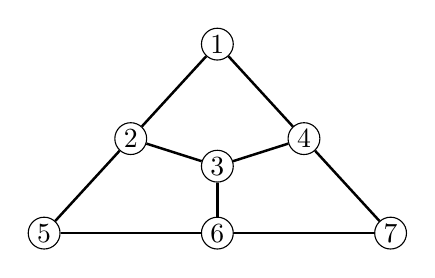
\begin{tikzpicture}[scale=1,
  every node/.style={circle, draw, fill=white, inner sep=1.2pt},
  e/.style={line width=0.9pt}
]

% --- triangle corners ---
\node (1) at (0,2.4) {1};
\node (5) at (-2.2,0) {5};
\node (7) at ( 2.2,0) {7};

% --- place 2,4,6 exactly on the triangle sides ---
% 2 on line segment 5--1, 4 on 1--7, 6 on 5--7
\node (2) at (-1.1,1.2) {2};
\node (4) at ( 1.1,1.2) {4};
\node (6) at (0,0) {6};

% interior node
\node (3) at (0,0.85) {3};

% --- outer triangle boundary as segmented sides ---
\draw[e] (5)--(2)--(1);
\draw[e] (1)--(4)--(7);
\draw[e] (5)--(6)--(7);

% --- interior edges (same as the original structure) ---
\draw[e] (2)--(3)--(4);
\draw[e] (3)--(6);

\end{tikzpicture}
\end{center}
where the stablizer codes are given by looking at the loops of the graph.
\begin{align}
    g_1 &= X_1X_2X_3X_4 \\
    g_2 &= X_2X_3X_5X_6 \\
    g_3 &= X_3X_4X_6X_7  \\
    g_4 & =Z_1Z_2Z_3Z_4 \\
    g_5 &= Z_2Z_3Z_5Z_6 \\
    g_6 &= Z_3Z_4Z_6Z_7  
\end{align}
Is this a valid $S$? Yes, because all the generators commute because there is an even amount of overlapping of $X$'s and $Z$'s. This is because they share edges. \\
$n=7, k=1$ logical qubits. ($n - \text{min \# of generators} = k$) \\
How many possible single-qubit Pauli errors are there? $7\cdot 3 + 1 = 22$ where 1 comes from identity. \\
The number of possible syndrome values is $2^6 = 64$. \\
This is the $[[7,1]]$ \textbf{Steane code}. 
\end{example}

\textit{For a valid stabilizer, $S$ needs to be an Abelian group, and all of its elements commute with each other, and it is sufficient that the generators all commute with each other.}


\begin{example}
    Let $S = \langle XZZXI, IXZZX, XIXZZ, ZXIXZ\rangle$. Then $n=5, k = 1$. This is the $[[5,1]]$ code. There are $5\cdot 3 + 1 = 16$ possible single qubit errors. The number of possible syndrome values is 16, since we have 1 bit for every single generator, and we have 4 bits and $2^4 = 16$. This is called the \textbf{perfect code}, which is the minimum amount of syndromes needed to distinguish all possible single bit errors. 
\end{example}
Quantum Hamming Bound: says that the number of syndrome bits must be at least equal to the number of single qubit errors that happen 
\begin{equation}
    \sum_{j=0}^t 3^j {{n}\choose{k}} \leq 2^{n-k}
\end{equation}
There are other perfect quantum codes: there is a family of these
\begin{equation}
    \left[\left[\frac{4^r -1}{3}, \frac{4^r-1}{3}-2r\right]\right]
\end{equation}
For $r=2, [[5,1]]$ and for $r=3, [[21,15]]$. \\

Stabilizer code properties: 
    \begin{definition}
        weight: for $g \in G$, $wt(g) = \text{\# of non-identity terms in the tensor product expansion}$
    \end{definition}
    \begin{definition}
        distance: 
        \begin{equation}
            d = \min_{E \in G_n, uncorrectible}[w(E)]
        \end{equation}
        s.t. $\braket{\psi_i|E|\psi_j} \neq \delta_{ij} \; \forall \ket{\psi_i} = V_s$, in other words this is the minimum weight of an uncorrectable/undetectable code (smallest error that makes you confused)
    \end{definition}
Weight is about a Pauli string; distance is about a code. \\
We use this distance in the nomenclature $[[n,k,d]]$. \\
For example, the $[[5,1]]$ is actually $[[5,1,3]]$ code since it detects a single qubit error, 3 possible errors. For example: $000,111$ is a [[3,1,3]] code (classical).  \\

\subsection{Classical Linear Codes}
A $[n,k]$ (classical) code is a set of bit strings. \\
Encodes a $k$-bit vector $\Vec{x} \rightarrow F_2^n$ into a $n$-bit vector \\
Recall: $[n,k,d]$ classical code encodes $k$ bits in $n$ bits with distance $d$ \\
Distance $d$ here is Hamming distance $d = \min(d(c_1,c_2)) : c_1, c_2 \in C $
\begin{definition}
    The $n \times k$ generator matrix $G$ encodes data $\vec{x}$ into $\vec{v} = G \vec{x}$ (columns of $G$ are basis codewords)
\end{definition}
\begin{example}
    $G = \begin{pmatrix} 1 \\ 1 \\ 1 \end{pmatrix}$, then $G \begin{pmatrix} 0 \end{pmatrix} = \begin{pmatrix} 0 \\ 0 \\ 0 \end{pmatrix}$ and $G \begin{pmatrix} 1 \end{pmatrix} = \begin{pmatrix} 1 \\ 1 \\ 1 \end{pmatrix}$
\end{example}
\begin{definition}
    The parity check matrix $H$ is an $n - k$ by $n$ matrix s.t. $H\vec{v} = 0 \forall \vec{v} \in C$, $C$ is codespace. Equivalently, $HG=0$ because the columns of $G$ are codewords (defines nullspaces). $H$ is an $(n-k) \times n$ matrix and $G$ is an $n\times k$ matrix. 
\end{definition}
\begin{example}
    From the previous example, $\begin{pmatrix} 0 & 1 & 1 \\ 1 & 1 & 0 \end{pmatrix}$. This checks the parity of the right/left hand bits. The rows of $H$ must be perpendicular to columns of $G$.    
\end{example}
\begin{definition}
    Let $C$ be an $[n.k]$ code with generator $G$, and parity check matrix $H$. Then we define $C^\perp$ is the code with generator $H^T$ and parity check matrix $G^T$. $C^\perp$ is the dual code. 
\end{definition}


\subsection{CSS Codes}
Calderbank, Shor, Steane - CSS Codes is a family of good $[[n,k,d]]$ codes correcting $t$ errors. 
\begin{definition}
    CSS codes (quantum) \textit{We'll be using two classical codes to create one quantum code}\\ 
    Let classical codes $C_1$ be $[n,k_1]$ and $C_2$ be $[n,k_2]$ s.t. $C_2 \subset C_1$, \textit{That is, all the codewords in $C_2$ are also in $C_1$, thus $C_1$ can correct for everything inside $c_2$}, and $c_1$ and $c_2^\perp$ both correct $t$ errors i.e. $H_2 = H(c_2^\perp) = G_2^T$ corrects $t$ errors. Then the code $CSS(C_1,C_2)$ is defined by the following stabilizers which is generated by 
    \begin{equation}
        S = \langle X[H_2], Z[H_1] \rangle 
    \end{equation}
    where $X[\cdot] = \text{replace } 0 \rightarrow I, I\rightarrow X$ and $Z[\cdot] = \text{replace } 0 \rightarrow I, I\rightarrow Z$, and take rows as generators $Rightarrow$ binary notation (binary symplectic matrix representation of a CSS code): 
    \begin{equation}
        \left(\begin{array}{c|c} X & Z \end{array}\right)= \left(\begin{array}{c|c} G_2^{T} & 0\\ \hline 0 & H_2 \end{array}\right)
    \end{equation}
\end{definition} 
$H_2 =$ parity check matrix of $c_2^\perp$ \\ 
$H_1 =$ parity check matrix of $c_1$ \\
$CSS(c_1,c_2)$ has parameters $[[n,k_1-k_2]]$ \\
Is $S$ a valid stabilizer? YES, need elements to commute. This implies that we need $H_2H_1^T = 0$. \\
\begin{equation}
     H_2H_1^T = H(C_2^\perp)H_1^T = G_2^TH_1^T = (H_1G_2)^T = 0
\end{equation}
since $H_1G_1 = 0$ by definition of the parity check matrix and $G_2$ is the set of codewords and $C_2$ is a subspace of the codewords in $G_1$. \\

CSS code idea: $C_1$ corrects bit flips errors ($X$ errors).  This is because $Z[H_1]$ is the parity check matrix for $C_1$ and we made $Z$ stabilizer strings out of it, which anti-commute with $X$ errors. $C_2$ corrects phase flips errors ($Z$ errors). This is because $X[H_2]$ is the parity check matrix for $C_2$ and we made $X$ stabilizer strings out of it, which anti-commute with $Z$ errors. 
\begin{equation}
    CSS(c_1,c_2) = \{\ket{X + c_2} = \frac{1}{\sqrt{\norm{c_2}}} \sum_{y \in c_2} x+y \,|\, \forall x \in C_1\}
\end{equation}


Group picture: $c_2 \subset c_1$, What happens if we add a number to $C_2$? In group theory, if we multiply all the elements of a subgroup by an element of that subgroup, we get a coset. each one of these $\ket{x+c_2}$ is like a coset. $c_1$ corrects bit flips and $c_2$ corrects phase flips. Each coset is a distinct codeword. 

\begin{example}
    $[[7,1,3]]$ is a CSS code. (Here $c_2 = c_1$). \\
    $[[9,1,3]]$ is a CSS code. \\
    $[[5,1,3]]$ is not a CSS code. \\
\end{example}